\documentclass[table,xcdraw]{article}
\usepackage[table,xcdraw]{xcolor}
\usepackage{graphicx}
\usepackage{float}
\usepackage{todonotes}
\usepackage{caption}
\usepackage{multirow}
\usepackage{hyperref}

\begin{document}

\title{CS598 - Data Mining Capstone\\
		\large Task 7 - Word2Vec Explorer}

\author{Rodrigo Rodrigues}
\date{May 15th, 2020}
\maketitle


\abstract{For this task we should focus on one application or technique utilized during the semester and develop a web application to allow others experiment with the tool. For this I have chosen Word2Vec for identifying related words on a text corpus. I have experimented with this algorithm in task 3 and have achieved good results for identifying words in the same category as the pre-tagged labels.}

\section{Introduction}

Word2Vec is a word embedding that uses a vector space for representation and is very efficient in identifying relationship between words.
This web Application, named Word2Vec Explorer, is a way of exploring a text data set and the Word2Vec text representation and understanding how the technique works. The interface provides a way of training models with Word2Vec using different parameters and datasets and exploring the results on a interactive graph plot as well as a drill down table by word.


The application can be accessed in the following url:

\href{http://word2vec-explorer.azurewebsites.net/}{http://word2vec-explorer.azurewebsites.net/}

The source code is available in this github repository:

\href{https://github.com/serdasteclas/CS598-T7}{https://github.com/serdasteclas/CS598-T7}

\section{Exploring Models}

At the start page of the application you are presented with a list of the available models, selecting one of the models will display information about the datasets and the parameters used in training the model.

\begin{figure}[H]
	\centering
	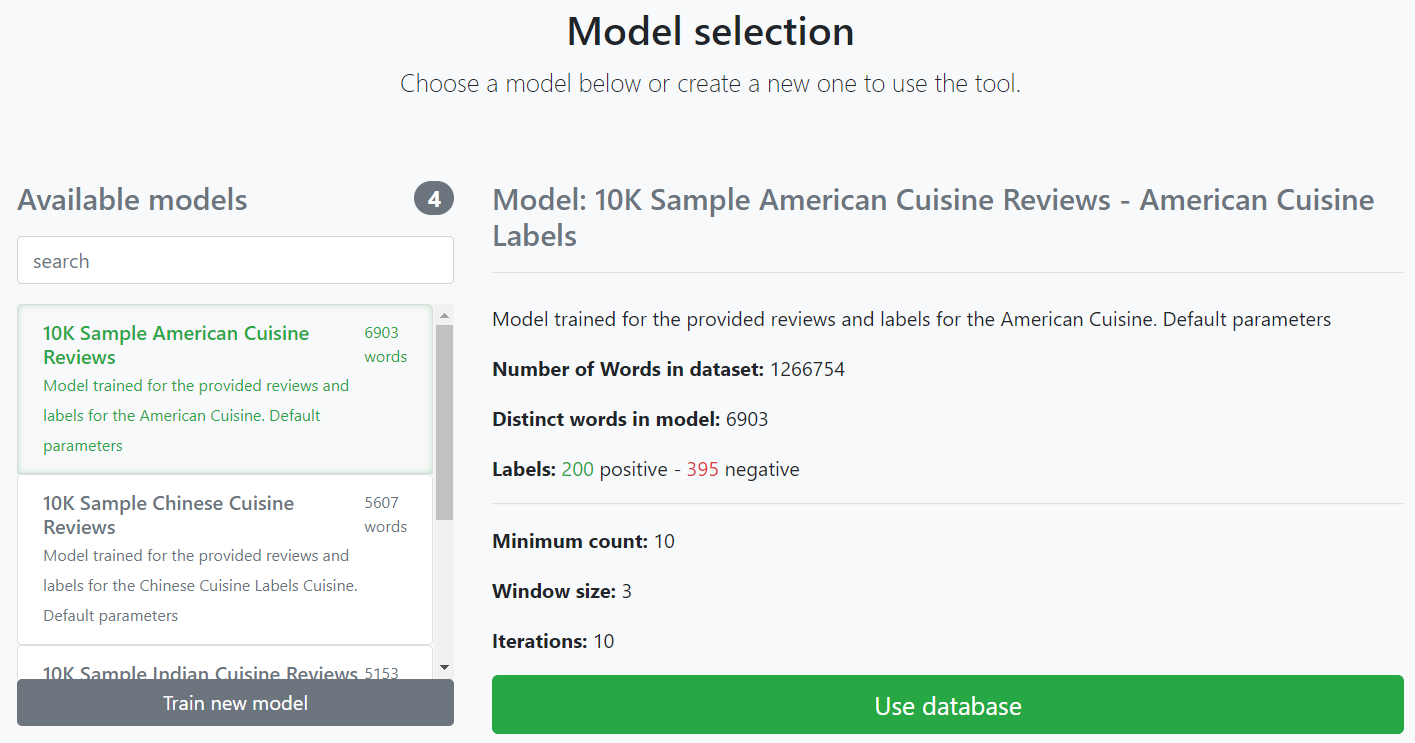
\includegraphics[width=\linewidth]{screen_model_list}
	\caption{Model List}
	\label{fig:screen_model_list}
	\end{figure}

Selecting the model and clicking on "Use database" will open the visualization for the model.
In this section the user is presented with the name of the Dataset and Label files, a threshold selector and a list of words.

The list of words contains the 1,000 words that are most similar to the positive labels of the label file and a similarity measure regarding the positive labels. This can be used for finding words of a specific category. In the Task 3, I used this to find dishes in the reviews from the Yelp dataset, this can be easily done in this tool, the provided labels and a sample of the reviews from each cuisine provided in task 3 is preloaded on the tool for testing.
An example of a similar use case would be mining actors in a movie review dataset or products in an e-commerce website.

Selecting a word from the list on the left will open a second list and render the interactive graph representation.
The first list shows the top 1,000 related to the label list while the second list shows the top 200 words related to the word selected on the first list.

\begin{figure}[H]
	\centering
	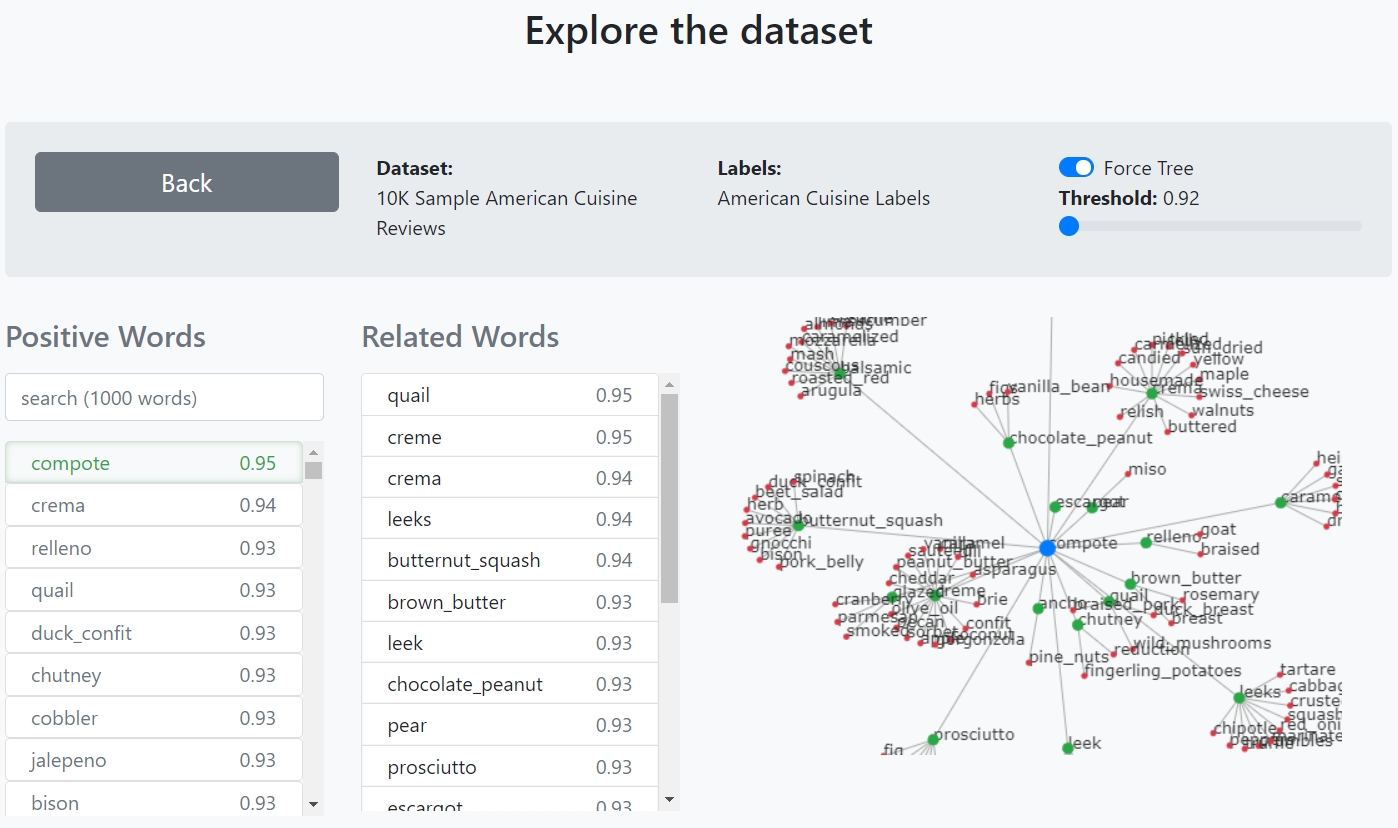
\includegraphics[width=\linewidth]{screen_explore_model}
	\caption{Exploring model}
	\label{fig:screen_explore_model}
	\end{figure}

On the right top of the screen a threshold slider can be used to adjust the elements displayed on the graph. The slider will be automatically adjusted to match the range of the second list. For a different visualization the toggle switch can be activated, this will force the graph to render as a tree, disconnecting the links between sub-branches. The graph represents a third level of relations not visible on the lists.

\begin{figure}[H]
	\centering
	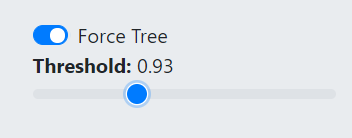
\includegraphics{screen_threshold}
	\caption{Graph controls}
	\label{fig:screen_threshold}
	\end{figure}


\section{Training Models}

On the training screen the user can upload a new dataset and label file or use one of the available files.

\begin{figure}[H]
	\centering
	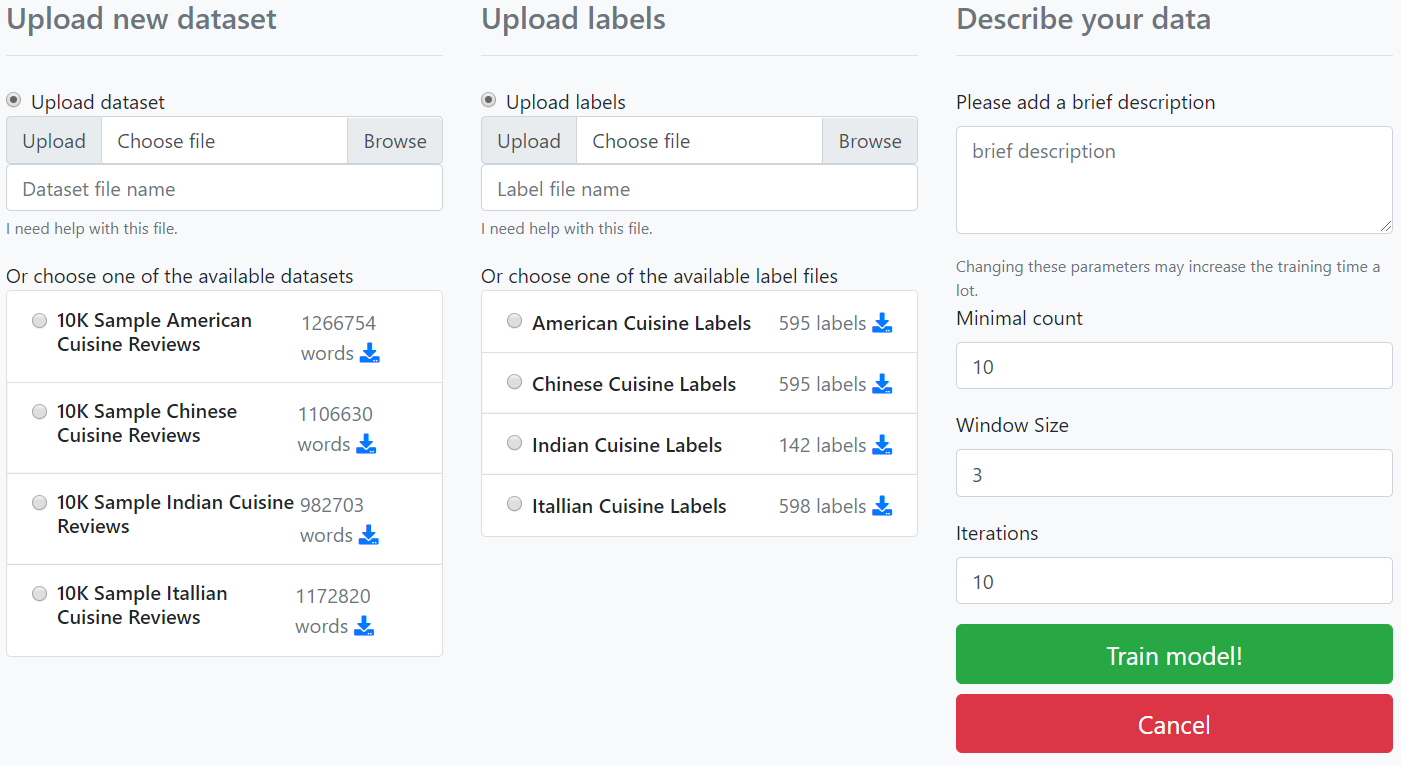
\includegraphics[width=\linewidth]{screen_train_new_model}
	\caption{Train New Model}
	\label{fig:screen_train_new_model}
	\end{figure}

When uploading a file, a name for the new file is required and the field bellow the upload component must be filled.
To make easier for the user to understand the format of the files, there is a help screen for each file that can be accessed by clicking on the the message "I need help with this file.". The uploaded files can also be downloaded by clicking the download icon near the stats of each file. Please note that for storage reasons files with the same md5 hash are considered duplicates and discarded, to easily implement this I choose to save the file with the hash as name, so the original filename is lost in the processes and all files are renamed to their own hash, to open in a text editor it may be necessary to add the '.txt' extension to the file.

The main dataset (i.e., the reviews on the Yelp scenario) must be a plain text file with one document in each line. The labels must contain a label per line and a positive or negative indicator separated by a tab character, exactly as in the files provided for Task 3.

\begin{figure}[H]
	\centering
	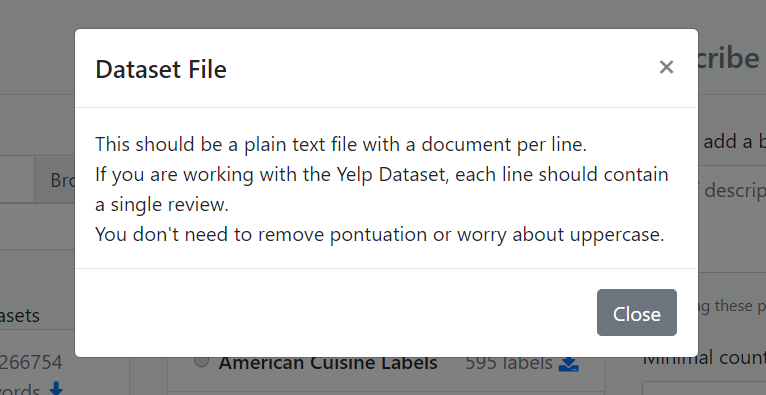
\includegraphics[width=\linewidth]{screen_help_dataset}
	\caption{Dataset Instructions}
	\label{fig:screen_help_dataset}
	\end{figure}

\begin{figure}[H]
	\centering
	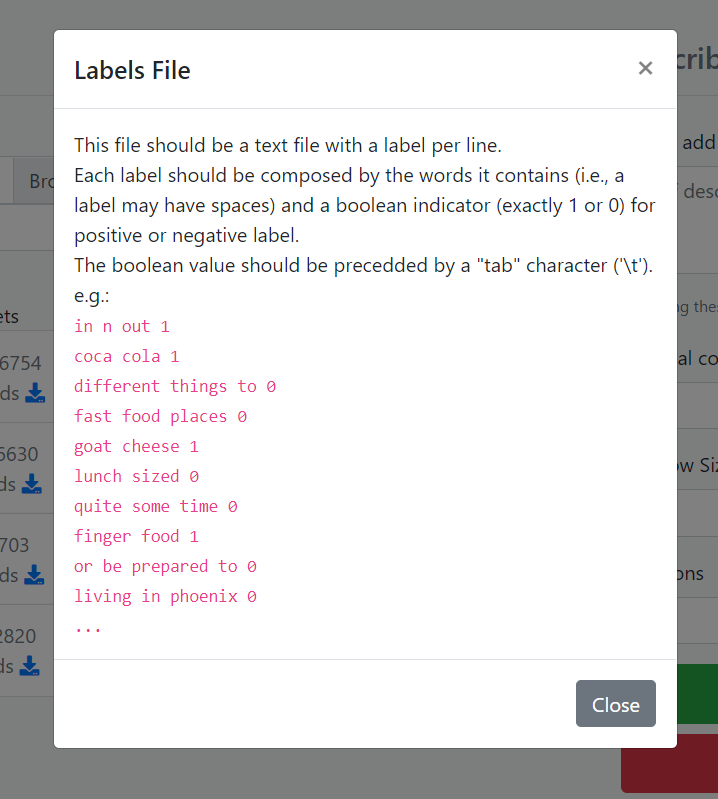
\includegraphics[width=\linewidth]{screen_help_labels}
	\caption{Label Instructions}
	\label{fig:screen_help_labels}
	\end{figure}

A brief description for the model is required, this description will be displayed on the listing in the front page of the application.

In this screen the user can also chose the parameters for the model training (Minimal count, window size and number of iterations).

After filling all the fields and clicking the "Train model!" button, the user is redirected to a status page that will display a summary of the model and a processing animation, this pages refreshes automatically and the user just have to wait.

\begin{figure}[H]
	\centering
	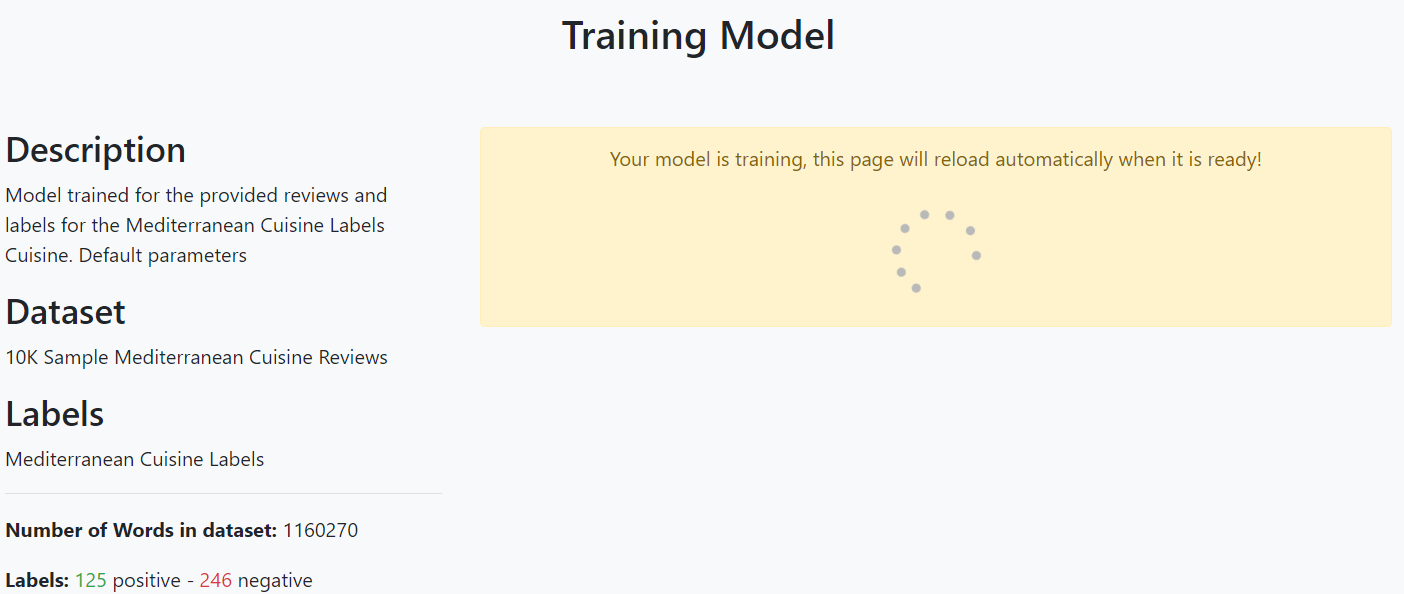
\includegraphics[width=\linewidth]{screen_model_training}
	\caption{Model Training}
	\label{fig:screen_model_training}
	\end{figure}

After the training is complete, the user is presented with a confirmation message and a direct link to the model. Note that changing the parameters may increase the training time significantly. Training the models on these datasets on this server usually takes less than two minutes.


\begin{figure}[H]
	\centering
	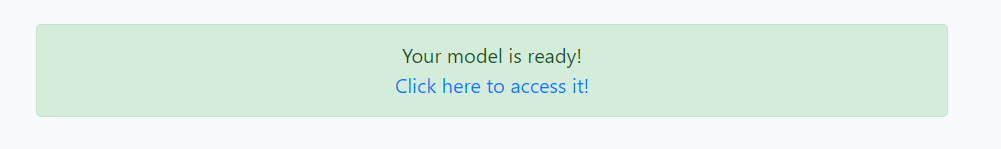
\includegraphics[width=\linewidth]{screen_trainin_done}
	\caption{Model Trained}
	\label{fig:screen_trainin_done}
	\end{figure}

For usability I've added a search function to the most important lists and friendly error messages.

\section{Technology Stack}

The application is written in python and uses Flask as web framework, there is no feature that is dependent of any specific cloud service and the application can be run locally.
For the database I initially used a SQLite file, this option is still available in the code though the SQLAlchemy object-relational mapper and is great for testing locally, but for production I decided to deploy using an Azure SQL Database to avoid problems with concurrency.
The interface is mostly based on Bootstrap 4, and JQuery, the graph interactive plot was made using D3.js.

\section{Conclusion}

This assignment gave me an opportunity to learn how to deploy a web application using python, something I had never tried before.
I am not aware of other web based tool for training and exploring Word2Vec models without the need of writing code, that is also free and open source.
For improving over this project I would suggest adding more models, different parameter customizations and better plots.


\end{document}